\documentclass{article}
\usepackage[utf8]{inputenc}
\usepackage{datetime}
\usepackage{enumerate}
\usepackage{textcomp}
\usepackage{amsmath}
\usepackage{tikz}
\usetikzlibrary{arrows}
\usepackage{graphicx}
\usepackage{amssymb}
\graphicspath{ {./images/} }
   
\title{\bf \Large ASSIGNMENT 12}
\author{Xinhao Luo}
\date{\today}

\def\math#1{$#1$} 

\setlength{\textheight}{8.5in}
\setlength{\textwidth}{6.5in}
\setlength{\oddsidemargin}{0in}
\setlength{\evensidemargin}{0in}
\voffset0.0in

\begin{document}
\maketitle
\medskip

\section{Neural Networks and Backpropagation}

\begin{enumerate}[a)]
    \item Reports
        \begin{itemize}
            \item [Identity] Layers
                \begin{enumerate}[1)]
                    \item \math{\begin{bmatrix}
                            -0.01938197 & -0.01938197 \\
                            -0.01938197 & -0.01938197 \\
                            -0.03876394 & -0.03876394 
                        \end{bmatrix}}
                    \item \math{\begin{bmatrix}
                            -0.18460146 \\
                            -0.14059139 \\
                            -0.14059139 
                        \end{bmatrix}}
                \end{enumerate}
            \item [Tanh] layers
                \begin{enumerate}[1)]
                    \item \math{\begin{bmatrix}
                            -0.01594156 & -0.01594156 \\
                            -0.01594156 & -0.01594156 \\
                            -0.03188311 & -0.03188311 
                            \end{bmatrix}}
                    \item \math{\begin{bmatrix}
                            -0.15183362 \\
                            -0.1156356 \\
                            -0.1156356 
                        \end{bmatrix}}
                \end{enumerate}
        \end{itemize}
    \item The result are identical to a) 
        \begin{itemize}
            \item [Identity] Layers
                \begin{enumerate}[1)]
                    \item \math{\begin{bmatrix}
                            -0.01938197 & -0.01938197 \\
                            -0.01938197 & -0.01938197 \\
                            -0.03876394 & -0.03876394 
                        \end{bmatrix}}
                    \item \math{\begin{bmatrix}
                            -0.18460146 \\
                            -0.14059139 \\
                            -0.14059139 
                        \end{bmatrix}}
                \end{enumerate}
            \item [Tanh] layers
                \begin{enumerate}[1)]
                    \item \math{\begin{bmatrix}
                            -0.01594156 & -0.01594156 \\
                            -0.01594156 & -0.01594156 \\
                            -0.03188311 & -0.03188311 
                            \end{bmatrix}}
                    \item \math{\begin{bmatrix}
                            -0.15183362 \\
                            -0.1156356 \\
                            -0.1156356 
                        \end{bmatrix}}
                \end{enumerate}
        \end{itemize}
\end{enumerate}

\section{Neural Network for Digits}

\begin{enumerate}[a)]
    \item 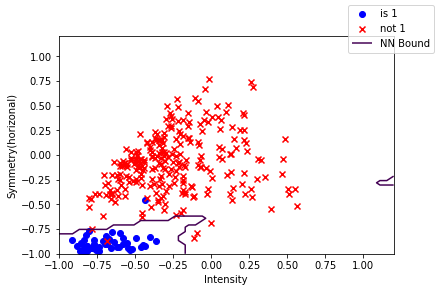
\includegraphics[]{2/42} \\ 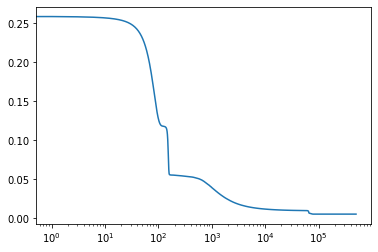
\includegraphics[]{2/21}
    \item 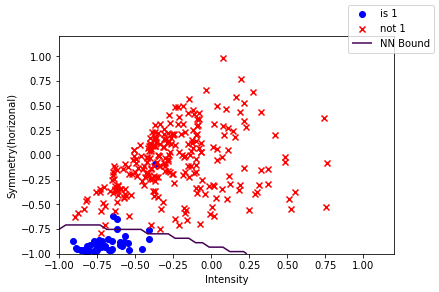
\includegraphics[]{2/62}
    \item 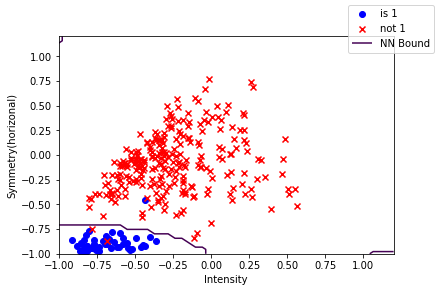
\includegraphics[]{2/52}
\end{enumerate}

\section{Support Vector Machines}

\begin{enumerate}[a)]
    \item For the two point \math{(1, 0)} and \math{(-1, 0)}, the line segment go through them is \math{x_2 = 0}, as well as the midpoint \math{(0, 0)}. The optimal hyperplane will be perpendicular and pass the midpoint, which is \math{x_1 = 0}
    \item \begin{enumerate}[i)]
        \item \math{z_1 = [1, 0]}, \math{z_2 = [-1, 0]}
        \item The line segment go through is \math{z_2 = 0}, so we have \math{z_1 = 0} as the optimal hyperplane.
    \end{enumerate}
    \item 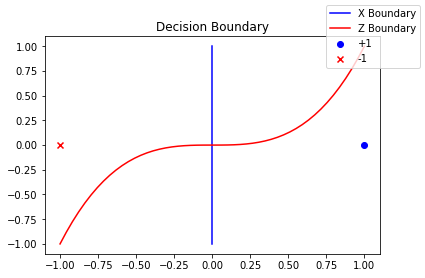
\includegraphics[]{3/1}
    \item \math{K(x, y) = z(x)z(y) = (x_1^3-x_2, x_1x_2)(y_1^3-y_2, y_1y_2) = x_1^3y_1^3 - y_2x_1^3 - x_2y_1^3 + x_2y_2 + x_1x_2y_1y_2}
    \item \math{g(x) = sign(x_1^3 - x_2)}
\end{enumerate}

\section{SVM with digits data}

\begin{enumerate}[a)]
    \item 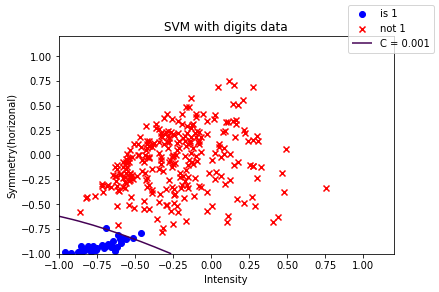
\includegraphics[]{4/1} \\ 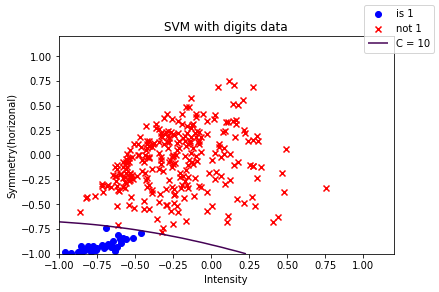
\includegraphics[]{4/2}
    \item When C is getting bigger, the decision boundary can be more complex and fit more data since more penalty applied on each misclassified data point. \math{E_in} also dropped when C increased, but it is believed that when C grows larger than optimal the performance increment will stop.
    \item \math{C = 1.9}, \math{E_{val} = 0.02} \\ 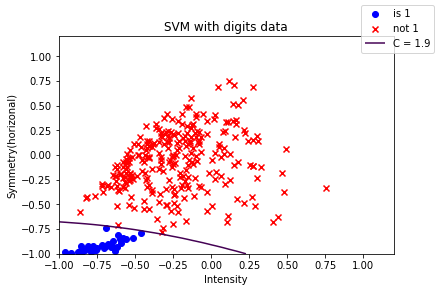
\includegraphics[]{4/3}
\end{enumerate}


\section{Compare Methods: Linear, Neural Network, SVM}

Comparing across the results of the algorithm listed above, all of them get a pretty good result (\math{\approx 2\%} test errors), pretty much the expected rate of this hand writing dataset. \\ However, among these algorithms, I would suggest SVM, considering its accuracy and speed to train. SVM comes with relative same performance as Neural Network but much significant lower computing cost. While for Linear model, it is lacking margin regularization featured in SVM, so its accuracy improved by choosing relative simple hypothesis thus may be limited. It is believed that SVM may be the best among three by providing reliable output with relative small computational requirements.

\end{document}
